\chapter{Resultados} \label{cap:resultados}


%%Nos parâmetros de previsão de consumo no ICT Unifesp, a função ReLu ganha destaque para utilização em neurônios nas camadas ocultas da rede neural, por ser simples e eficiente para a aplicação nos experimentos, visto que na fase feed-forward tem efeito parecido com a função identidade, e na fase feed-backward durante o reajuste dos pesos pelo otimizador, conforme ilustrado na Figura \ref{fig:ReLu}, sua derivada produz efeito degrau zerando valores negativos e sendo adequada na aplicação do domínio destes parâmetros, visto que todas as variáveis endógenas e exógenas utilizadas como parâmetros de predição, como por exemplo pressão atmosférica, vendas e consumo de dias anteriores, datas, entre outros, não possuem valores negativos. Já a função linear ganha destaque para aplicação no neurônio de saída que determina o consumo previsto para uma data no futuro, pois na fase feed-backward do reajuste dos pesos pelo algoritmo de treino backpropagation, a derivada da função linear se torna zero, fazendo com que o algoritmo de treino transforme apenas os pesos sinápticos dos parâmetros de entrada os pesos sinápticos dos neurônios nas camadas ocultas da rede, sem interferir no neurônio de saída.

Este Capítulo descreve os principais resultados experimentais obtidos durante esta pesquisa. Como descrito no Capítulo 4, os experimentos foram conduzidos em duas fases. Contudo, optou-se por apresentar neste Capítulo, apenas os principais resultados obtidos. Os demais resultados estão disponíveis nos Anexos deste documento. As primeiras seções introduzem a organização dos dados, uma breve análise das variáveis e o protocolo experimental, respectivamente.

\section{Organização do conjunto de dados}
%\TODO{descrever, nessa seção, como os dados foram organizados em treino, validação e teste}

    O procedimento de coleta de dados foi realizado de acordo com a metodologia da Seção \ref{subsec:coleta_endogenos} para os dados endógenos, e de acordo com os passos da Seção \ref{subsec:coleta_exógenos} foram obtidos os dados exógenos.
    Ambos os conjuntos de dados coletados foram estruturados conforme a Tabela \ref{table:dataset_final}, contendo um intervalo temporal de registros, desde o 12 de abril de 2017 (2017-04-12)  para o primeiro registro até o 16 de dezembro de 2019  (2019-12-16)  para o último registro, totalizando 514 registros de consumo de refeições em dias letivos.
    
    Conforme a metodologia definida na Seção \ref{subsec:fases_experimentais} este conjunto de dados com o total de 514 registros, foi duplicado para 2 fases experimentais distintas, cada fase com uma organização específica do conjunto de dados. O conjunto de dados da primeira fase experimental foi organizado de acordo com a Figura \ref{fig:case1_timeline}. Esta fase tem o conjunto de validação contemplando exclusivamente o primeiro semestre de 2018, indicando que o primeiro semestre de 2018 pudesse apresentar um movimento de consumo e vendas semelhante ao primeiro semestre de 2019, sendo a ideal para testes envolvendo somente o primeiro semestre do conjunto de testes.

    \begin{figure}[htb]
        	\center{        		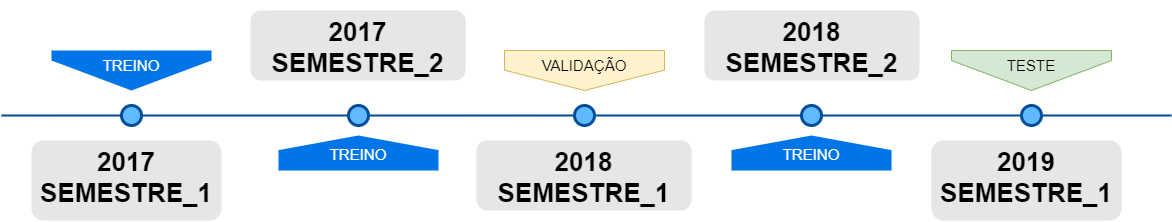
\includegraphics[width=1.0\textwidth]{./Figuras/resultados/case1_timeline.png}
        	 	\caption{Domínio temporal da fase 1.} \label{fig:case1_timeline} }
        \end{figure}
    Para a segunda fase o conjunto de dados foi organizado de acordo com a Figura \ref{fig:case2_timeline}. Para esta fase o conjunto de validação selecionado  contemplou o ano letivo de 2018 por completo, já para os experimentos de teste dos modelos os dados selecionados contemplaram o todo o ano letivo de 2019.
    
    \begin{figure}[H]
        	\center{        		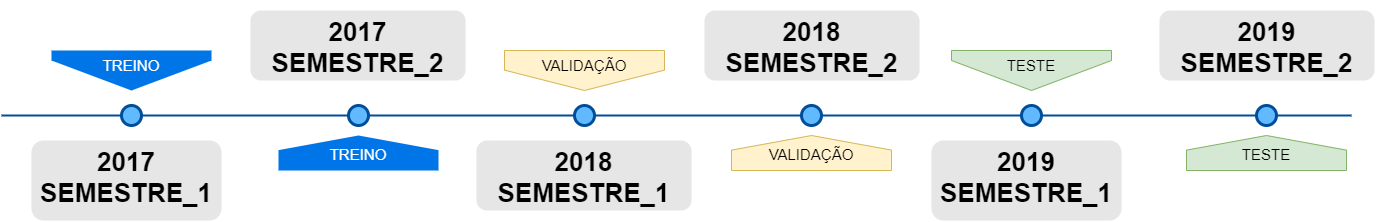
\includegraphics[width=1.0\textwidth]{./Figuras/resultados/case2/case2_dominio.png}
        	\caption{Domínio temporal da fase 2} \label{fig:case2_timeline} }
        \end{figure}
   
    %\paragraph{Dificuldades encontradas e resolvidas}
    \subsection{Manipulação e pré-processamento do conjunto de dados}
    
    Buscando organizar os dados brutos obtidos para a sua posterior aplicação nos modelos foram encontrados algumas peculiaridades. A primeira dificuldade encontrada nos experimentos foi um comportamento anômalo do resultados de previsão para o modelo RNN\_ENDO\_2. A linha azul na Figura \ref{fig:pandas_wrong_indexing} representa uma previsão refeições do modelo RNN\_ENDO\_2, e a linha vermelha valores reais de consumo do primeiro semestre de 2019. Com isto, foi possível observar que em ambos os conjuntos (real e predito) este comportamento estava presente. 
    
    \begin{figure}[!htpb]
    	\center{
    		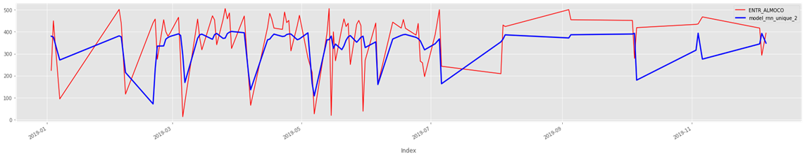
\includegraphics[width=1.0\textwidth]{./Figuras/resultados/pandas_wrong_indexing.png}
    	\caption{Resultado do modelo RNN\_ENDO\_2 obtido sobre o conjunto de dados aleatoriamente ordenado sobre o tempo.} \label{fig:pandas_wrong_indexing} }
    \end{figure}
    
    Após uma análise exploratória foi descoberto que os registros continham um erro na indexação por data, onde a estampa de datas se apresentava trocada, ou seja os dias por meses e vice-versa. Após a correção deste problema indexação os dados de consumo real e previsão produziram resultados realísticos e dentro do formato esperado, conforme apresentado na Figura \ref{fig:pandas_correct_indexing}, que apresenta um exemplo de predição pelo modelo RNN\_ENDO\_2 e os dados reais para o período do almoço.
    \begin{figure}[!htpb]
    	\center{
    		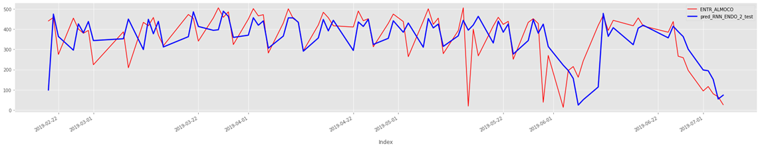
\includegraphics[width=1.0\textwidth]{./Figuras/resultados/pandas_correct_indexing.png}
    	\caption{Resultado do modelo RNN\_ENDO\_2 obtido sobre o conjunto de dados com ordenação corrigida } \label{fig:pandas_correct_indexing}}
    \end{figure}
              
\section{Avaliação das Variáveis}
Nessa Seção serão feitos alguns comentários em relação as características das variáveis que foram mais importantes para o problema, e serão apresentados alguns gráficos dos estudo estatístico feito para avaliar as relações entre elas. 

    \subsection{Estimativas de consumo do restaurante}
    
        A análise da técnica de estimação de consumo, realizada de forma subjetiva em relação ao consumo da semana anterior, utiliza-se do cálculo de 30\% de produção acima do consumo do quinto dia anterior. Este método de estimativa é foi adotado para tolerar descartes devido à existência de multa contratual por falta de refeições. Ainda, é possível observar que este modelo de 30\% a mais produz um comportamento linear, representado pela linha azul na Figura  \ref{fig:ru_pred},  estando distante do comportamento real de consumo, indicado pela linha vermelha. 

        \begin{figure}[!htbp]                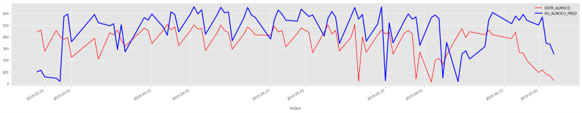
\includegraphics[width=\textwidth]{./Figuras/resultados/case1_ru_pred.png}
                \caption{Estimativa do restaurante para o ano de 2019.} \label{fig:ru_pred} 
        \end{figure}

            
        
        Apesar da estimativa seguir as tendências de quedas e aumento de consumo, a Figura \ref{fig:ru_pred_scatter} apresenta a dispersão gerada entre a estimava do R.U e o consumo real no ano de 2019, demonstrando que a regressão linear (linha vermelha) tem o eixo totalmente descentralizado com a função identidade da estimativa ideal (representada pela diagonal imaginária formada entre a origem do gráfico e o vértice superior direito). 
        

                \begin{figure}[ht]
                    \center{                    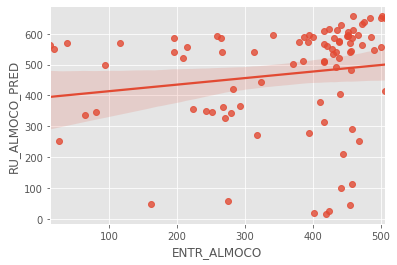
\includegraphics[width=0.6\textwidth]{./Figuras/resultados/case1_ru_pred_scatter.png}
                    \caption{Gráfico de dispersão da estimativa de consumo do restaurante para o ano de 2019.} \label{fig:ru_pred_scatter} }
                \end{figure} 

        
        
        Assim esse formato de predição gera também um erro maior do que 30\% no somatório total de refeições descartadas no semestre, ocasionado pelo comportamento oscilatório do consumo, conforme a Tabela \ref{table:case2_rupred}.

            \begin{table}[!ht]
            \centering
            \rowcolors{2}{gray!25}{white}
                \begin{tabular}{c|c}
                \rowcolor{gray!50}
                \hline
                \multicolumn{2}{c}{Consumo com margem 30\% acima do 5o dia anterior}\\ \hline     
                TOTAL DE REFEIÇÕES CONSUMIDAS & 58653  \\
                TOTAL DE REFEIÇÕES ESTIMADAS & 76262 \\ 
                CORRELAÇÃO (r)&  0.4006 \\
                P-value & 2.0845e-08\\
                RMSE & 191.7620 \\
                SOMA DOS ERROS POSITIVOS & 23412 \\
                SOMA DOS ERROS NEGATIVOS & -5803 \\
                ERRO ABSOLUTO MEDIANO & 133.0 \\
                ERRO ABSOLUTO PERCENTUAL MEDIO & 205.6113\% \\  \hline 
                \end{tabular} \caption{Métricas da estima de consumo do restaurante para o ano de 2019}
            \label{table:case2_rupred}
            \end{table}

    \subsection{Análise das variáveis endógenas}
    
        As variáveis endógenas são os parâmetros temporais de entrada nos modelos MLP e GRU, correspondentes ao domínio de consumo no restaurante.
         % \newpage
        \subsubsection{Consumo do dia vigente em relação às vendas de tickets do dia anterior}
        
        É possível notar na Figura \ref{fig: case1_consumo_vendas_almoco} que as vendas de \textit{tickets} no período de almoço apresentaram comportamento diferente no ano de 2017 em comparação aos anos seguintes devido à uma limitação imposta pelo restaurante, a partir de 2018 os alunos poderiam adquirir apenas 2 tickets por dia. Possivelmente, esta limitação foi dada para aproximar o comportamento de consumo de 1 ou 2 dias seguintes à venda do ticket. Esta limitação pode ser interpretada como método de auxílio à gestão para a produção de refeições e para o tratamento de desperdício.
        
        \begin{figure}[h]
                    	\center{                    		        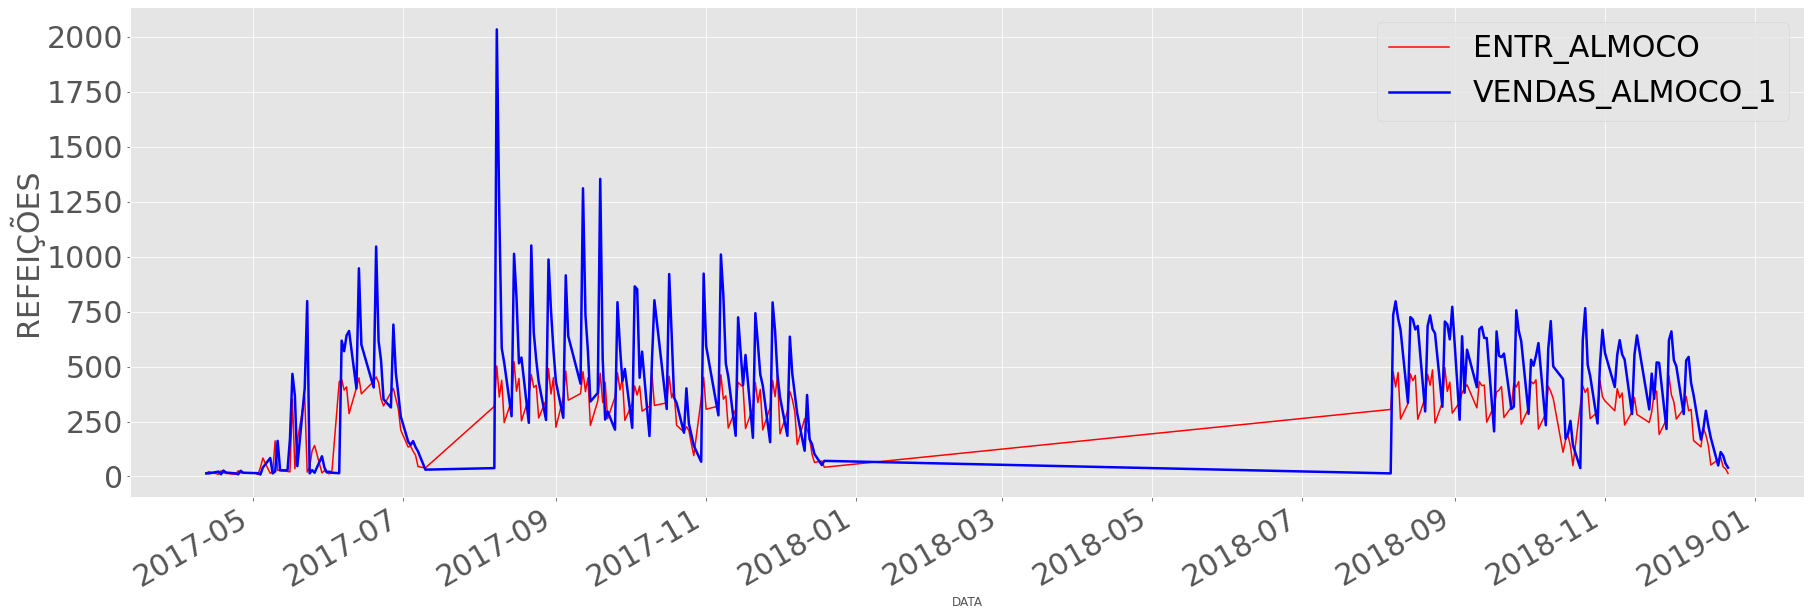
\includegraphics[width=0.8\textwidth]{./Figuras/resultados/case1_consumo_vendas_almoco.png}
                    	\caption{Correlação entre consumo e vendas de almoço.} \label{fig: case1_consumo_vendas_almoco} 
                    	}
                    \end{figure}
	        
        Mesmo com o valor \textit{outlier} de 2000 vendas em um único dia, e com a nova limitação de compras de \textit{tickets} a partir de 2018, o consumo no horário de almoço está fortemente relacionado com as vendas de \textit{tickets} no período do almoço de um dia anterior. Nota-se também que os alunos se adaptaram à limitação imposta para utilização dos \textit{tickets} com prazo de validade de apenas dois dias, conforme o valor do coeficiente de correlação é de aproximadamente em 72\%, como apresentado na Tabela \ref{table:case1_vendas1}.
        
 \begin{table}[!htpb]
           \centering
           \caption{Comparação de consumo com um dia anterior}
             \rowcolors{2}{gray!25}{white}
             \begin{tabular}{c|c}\hline
                \multicolumn{2}{c}{CONSUMO EM RELAÇÃO ÀS VENDAS DE 1 DIA ANTERIOR}\\ \hline
                CORRELAÇÃO (r) &  0.7255528038157009\\
                P-value &5.399561176138223e-41\\
                RMSE & 260.5399426736619\\
                ERRO ABSOLUTO MEDIANO & 139.0\\
                ERRO ABSOLUTO PERCENTUAL MEDIO & 90.18\\\hline
            \end{tabular} \label{table:case1_vendas1} \end{table}
    	            

        
        Há outros fatores não previstos envolvidos, como possíveis falha de registros de vendas no sistema, bem como o valor \textit{outlier} de 2000 vendas pode ser interpretado com a migração de sistema e banco de dados de refeições que ocorreu em 2017 da unidade Talim do ICT-Unifesp para o banco de dados do Hospital São Paulo. Possivelmente também foram importadas vendas do sistema antigo sem a diferenciação de datas.
        
        A soma das vendas de refeições no horário do almoço, obteve um total de 242282 para todos os 514 registros no conjunto de dados. Neste mesmo período o valor real de consumo, ou seja alunos que efetivamente ingressaram no restaurante (passaram pela catraca) totalizou 163752 refeições. Apesar de notória, a diferença de 78.530 refeições vendidas acima do consumo real não foi passível de investigar neste trabalho. Ressaltando que estes valores foram obtidos no conjunto original de dados fornecidos pelo fiscal de contrato do R.U do ICT-Unifesp por meio de solicitação via e-mail para este fiscal.


                    \begin{figure}[!htpb]
                    	\center{                    		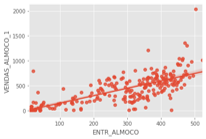
\includegraphics[width=0.7\textwidth]{./Figuras/resultados/case1_scatter_consumo_vendas_almoco.png}
                    	\caption{Gráfico de dispersão entre consumo e vendas de almoço.} \label{fig:case1_scatter_consumo_vendas_almoco} }
                    \end{figure}
                
                
          

            \subsubsection{Normalização e escala de \textit{features}}
            
                O processo de normalização e escala é demonstrado nesta Seção com a \textit{feature} de vendas de \textit{tickets} de 1 dia anterior, pois entre todas esta é a que produziu \textit{outliers} de maior destaque.
                A normalização dos dados é feita com o teto de 3x o desvio padrão médio, logo o pico de 2000 vendas foi normalizado para o valor arredondado de 1356 refeições. Mesmo com a normalização, o comportamento linear desta \textit{feature} se manteve, conforme apresentado na Figura \ref{fig:feature_sem_outliers}. 

                
                        \begin{figure}[H]
                        	\center{
                            	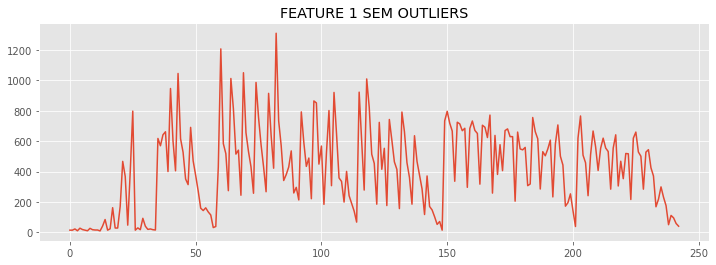
\includegraphics[width=0.9\textwidth]{./Figuras/resultados/feature_sem_outliers.png}
                            	\caption{Vendas de \textit{tickets} normalizados com teto de 3x o desvio padrão.}
                            	\label{fig:feature_sem_outliers}
                        	}
                        \end{figure}
                        
                        
                        Após a normalização foi realizada a padronização da escala de 0 a 1 nesta  e conforme é observado na Figura  \ref{fig:feature_sem_outliers_escalada}, o comportamento linear foi novamente mantido.
                        
                        \begin{figure}[H]
                        	\center
                        	{                    		
                            	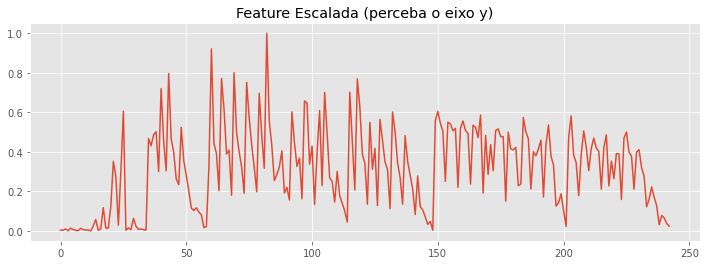
\includegraphics[width=0.9\textwidth]{./Figuras/resultados/feature_sem_outliers_escalada.png}
                            	\caption{Vendas de \textit{tickets} escalada entre 0 a 1.} \label{fig:feature_sem_outliers_escalada} 
                        	}
                        \end{figure}
                       
                Este processo de normalização e escala foi realizado para todas as métricas endógenas e também para as métricas climáticas.
        	   % \newpage
        	   
                \subsubsection{Consumo atual em relação ao consumo do jantar de 1 dia anterior.}
                %\TODO{QUILES - esse foi um dos fenômenos mais curiosos que encontrei e que não tenho explicação pra ele, o consumo da turma da noite é muito parecido com o consumo da turma do almoço do dia seguinte}
                
                %\TODOR{Isso não foi erro de carregamento dos dados? caso esteja tudo certo, pode deixar assim. De qualquer forma, mencione isso no texto como um achado.}
                Buscando encontrar e avaliar os possíveis relacionamento entre as diversas métricas utilizadas, esta análise ganhou destaque como um efeito anômalo e provavelmente casual encontrando entre os dados.
                Apesar das grades curriculares e horários dos alunos que consomem refeições no almoço serem, geralmente, dispares aos alunos que consomem o jantar na noite do dia anterior, nota-se uma relação evidente entre estas 2 variáveis.
                 Esse comportamento pode ser evidenciado pela congruência entre os parâmetros, como demonstrado na Figura \ref{fig:case1_consumo_jantar} e pela elevada correlação obtida na regressão linear (R = 0,7655) entre esses 2 consumos, apresentada na Figura  \ref{fig:case1_consumo_jantar_scatter}. Ainda que apresente uma relevante correlação, não foi possível determinar uma causa evidente para este efeito anômalo encontrado.

                
  
                \begin{figure}[H]
                	\center{
                	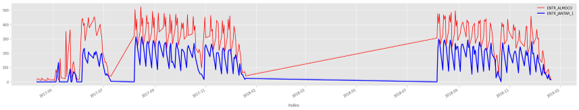
\includegraphics[width=0.8\textwidth]{./Figuras/resultados/case1_consumo_jantar.png}
                	\caption{Correlação de consumo de almoço e jantar de 1 dia anterior.} 
                	\label{fig:case1_consumo_jantar} }
                \end{figure} 
               
                \begin{figure}[H]
                	\center{                    		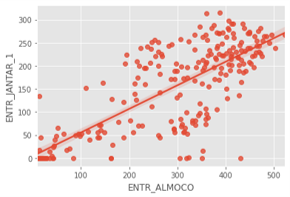
\includegraphics[width=0.8\textwidth]{./Figuras/resultados/case1_consumo_jantar_scatter.png}
                	\caption{Gráfico de dispersão entre consumo e jantar de 1 dia anterior.} 
                	\label{fig:case1_consumo_jantar_scatter} }
                \end{figure}
             
            
    	    \subsection{Análise da sazonalidade semanal}
    	        Os gráficos de consumo a seguir da Figura \ref{fig:case1_violinplot_segunda}, representando a segunda-feira,  até a Figura \ref{fig:case1_violinplot_sexta}, representando a sexta-feira, são gerados para as \textit{features} categóricas binárias, com a funcionalidade \textit{violin-plot} da biblioteca \textit{seaborn}, própria para distribuição de variáveis  categóricas binárias em um conjunto de dados.
    	        
    	        O violino azul com o valor 1 representa a distribuição do consumo ao longo do conjunto total de dados.
    	        O violino com valor zero pode ser ignorado e é um retorno padrão no gráfico da ferramenta, representando o complemento do consumo para o dia da semana considerado.
    	        Nas sextas feiras, o consumo teve escala de distribuição menor para todo o conjunto 2019. Foi notório que apesar da alternância de grades horárias durante a troca de semestres no ano de 2019, os dias de terça e quinta feira concentraram o maior movimento de consumo.
    	       %\newpage
    	      { \begin{center}    
    	        \begin{minipage}[c]{0.45\textwidth}
    	         \begin{figure}[H]
                	\center{                		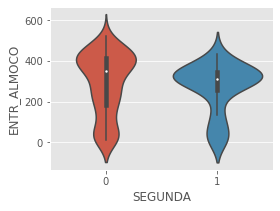
\includegraphics[width=\textwidth]{./Figuras/resultados/case1_segunda.png}
                	\caption{Gráfico de violino da distribuição do consumo na segunda feira.} \label{fig:case1_violinplot_segunda} }
                \end{figure}\end{minipage} \hfill %
                \begin{minipage}[c]{0.45\textwidth}
                \begin{figure}[H]
                	\center{                		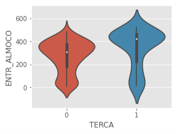
\includegraphics[width=\textwidth]{./Figuras/resultados/case1_terca.png}
                	\caption{Gráfico de violino da distribuição do consumo na terça feira.} \label{fig:case1_violinplot_terca} }
                \end{figure} \end{minipage}
                
            \begin{minipage}[c]{0.45\textwidth}
                \begin{figure}[H]
                	\center{                		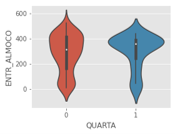
\includegraphics[width=\textwidth]{./Figuras/resultados/case1_quarta.png}
                	\caption{Gráfico de violino da distribuição do consumo na quarta feira.	} \label{fig:case1_violinplot_quarta} }
                \end{figure}\end{minipage} \hfill %
                \begin{minipage}[c]{0.45\textwidth}
                \begin{figure}[H]
                	\center{                		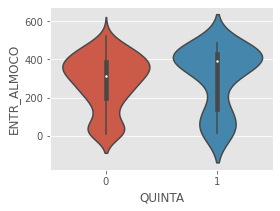
\includegraphics[width=\textwidth]{./Figuras/resultados/case1_quinta.png}
                	\caption{Gráfico de violino da distribuição do consumo na quinta feira.} \label{fig:case1_violinplot_quinta} }
                \end{figure}\end{minipage} %
                        \begin{minipage}[c]{0.45\textwidth}
                \begin{figure}[H]
                	\center{                		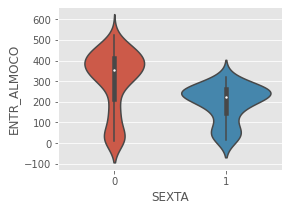
\includegraphics[width=\textwidth]{./Figuras/resultados/case1_sexta.png}
                	\caption{Gráfico de violino da distribuição do consumo na sexta feira.} \label{fig:case1_violinplot_sexta} }
                \end{figure}
                \end{minipage} \end{center} }
    \subsection{Análise das variáveis exógenas}
        As variáveis exógenas correspondem aos parâmetros, de domínio discreto, que são utilizados exclusivamente nos modelos de redes neurais mistos, e são lidos pelas camadas MLP destes modelos.
        
        \subsubsection{Consumo atual em relação ao avanço do semestre}
        
        Para esta análise foi necessário restringir o domínio de análise para 1 semestre, o consumo em relação ao avanço do semestre teve queda abrupta nos últimos dias do semestre, portanto a correlação dos conjuntos de dados das Figuras \ref{fig:case1_perc_sem} e \ref{fig:case1_perc_sem_scatter} obteve valor negativo.
        
                \begin{figure}[H]
                	\center{                    		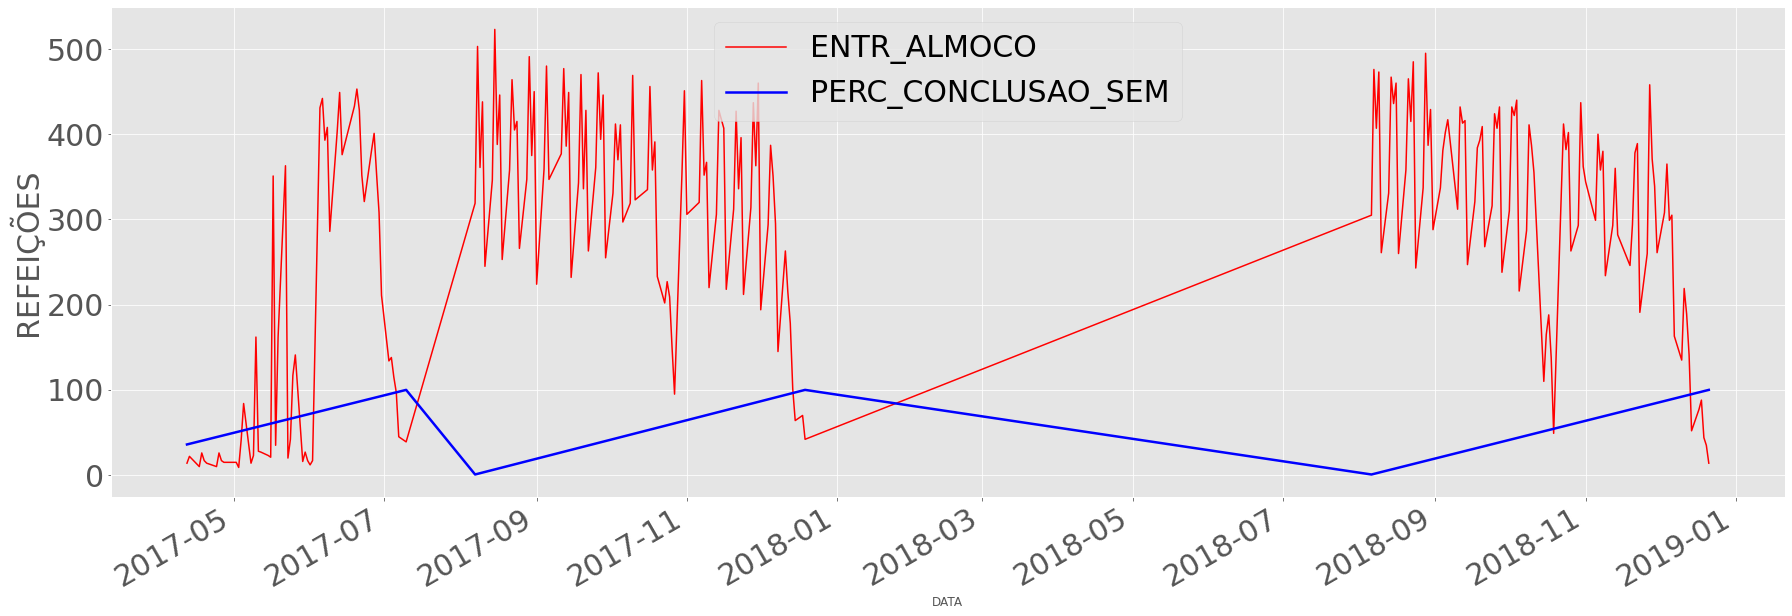
\includegraphics[width=\textwidth]{./Figuras/resultados/case1_perc_sem.png}
                	\caption{1a Fase : Relação da distribuição do consumo com o avanço do semestre, Correlação (r) = -0.35.}
                	\label{fig:case1_perc_sem}
                	}
                \end{figure}  

        
                       \begin{figure}[H]
                	\center{                		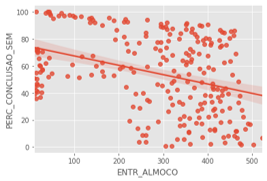
\includegraphics[width=\textwidth]{./Figuras/resultados/case1_perc_sem_scatter.png}
                	\caption{Gráfico de dispersão da distribuição do consumo com o avanço do semestre.} \label{fig:case1_perc_sem_scatter}
                	}
                \end{figure}
           

\section{Protocolo Experimental}
%\TODO{faça um resumo sobre as duas fases e as principais diferenças entre elas. Na sequência, detalhe os detalhes do principal modelo obtido (o com melhor resultado de predição)}
    Nesta Seção se iniciam os experimentos com os modelos de redes neurais.
    O primeiro experimento avalia o potencial de aprendizado dos modelos em  predizer o consumo do RU, por meio de um modelo básico de rede neural, ao concluir que as topologias mais básicas de redes neurais tem potencial de aprendizado sobre o problema foram desenvolvidas novas topologias.
    Em seguida, foi selecionado a topologia e a fase experimental que trouxe os melhores resultados e por fim a mesma é analisada e indicada como a solução final do trabalho.
    
    \subsection{Avaliação do aprendizado do problema da predição de refeições por meio de redes neurais MLP}
        \subsubsection{Ajuste empírico de topologia do primeiro modelo perceptron}
        
        O primeiro experimento com redes neurais realizado na primeira fase experimental, avaliou a capacidade de aprendizado do modelo perceptron sobre a sazonalidade dos dados endógenos, referentes ao domínio de consumo de refeições no R.U, verificando se o comportamento de consumo no restaurante pôde ser aprendido por este tipo de rede neural, portanto foi definida 1 rede neural inicial perceptron com apenas 1 camada oculta contendo 1 neurônio para 15 parâmetros de entrada (mesmo número de parâmetros endógenos) e com 1 neurônio de saída, denominada de MLP1.
        
        Os parâmetros endógenos correspondem à uma série temporal de intervalo de 5 dias anteriores para consumo de refeições no período do almoço, jantar e de vendas de \textit{tickets} no período do almoço.
        O modelo foi denominado MLP1, sua ilustração pode ser visualizada na Figura \ref{fig:case1_mlp1} obtida pela ferramenta NETRON. 
        
        \begin{figure}[H]
        \center{
        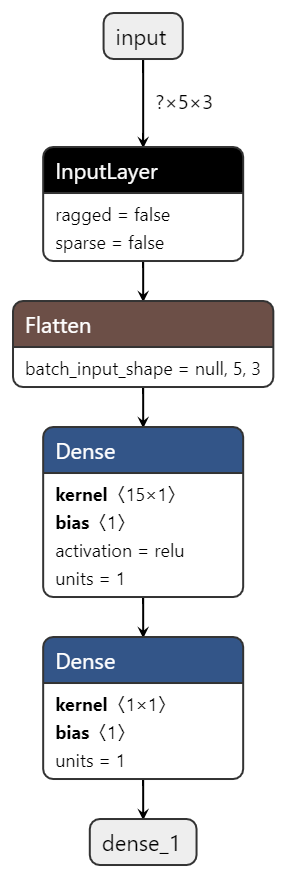
\includegraphics[width=0.3\textwidth]{./Figuras/resultados/case1_MLP1_validated.png}
        	\caption{Topologia do modelo MLP1, Ferramenta NETRON.} 
        	\label{fig:case1_mlp1}
        }
        \end{figure}
        
        
        Cada camada do modelo MLP1 corresponde à um bloco com título \textbf{Dense} nesta Figura, a primeira aresta da Figura entre o bloco \textit{input} e \textit{InputLayer} demonstra as 3 séries temporais dos parâmetros de entrada, com intervalo de 5 dias passados cada. \textbf{ENTR\_ALMOCO, ENTR\_JANTAR e VENDAS\_ALMOCO}. O bloco \textit{Flatten} converte cada dia de entrada das séries temporais em um parâmetro de entrada da rede neural MLP, conforme modelo conceitual do trabalho de \citeonline{Lopes2008} ilustrado na Figura \ref{fig:mlp-lopes} que utiliza apenas 1 parâmetro endógeno com intervalo temporal também de 5 dias. A primeira camada oculta desta rede pode ser visualizada no primeiro bloco dense da Figura que demonstra a função de ativação ReLu deste neurônio, e o número de unidades desta camada sendo 1.
        A camada de saída é o último bloco da Figura, também com 1 unidade, e como a função de ativação é linear, ela não é exibida na descrição do bloco.

        
        O treino deste modelo foi executado, obtendo RMSE com o valor 130,62 sobre o conjunto de validação, neste caso da primeira fase sendo os dados do primeiro semestre de 2018, e é possível notar na Figura \ref{fig:case1_mlp1_train} que as linhas da função de perda e treino demonstraram um treino adequado até a ultima época de treino, e como não houve uma aplicação de \textit{Validation Loss} simultânea com \textit{Train Loss}, o treino não produziu um \textit{overfitting}.
        \begin{figure}[H]
        	\center{
        	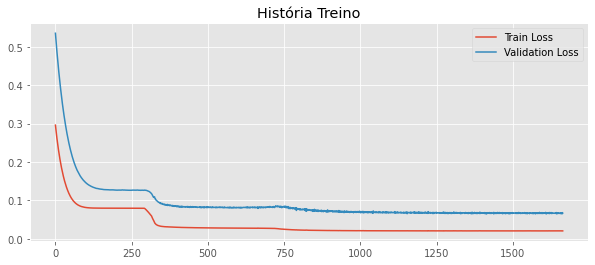
\includegraphics[width=0.8\textwidth]{./Figuras/resultados/case1_mlp1_train.png}
        	\caption{Gráfico de treino do modelo MLP1, RMSE = 130,62}
        	\label{fig:case1_mlp1_train}
        	}
        \end{figure}
        
        Portanto foi aumentada a profundidade do modelo MLP1 obtendo-se o modelo MLP2 com topologia ilustrada na Figura  \ref{fig:case1_mlp2}, e após o treino deste modelo foi possível notar a diminuição do RMSE para o valor de 107.97, como observado na Figura \ref{fig:case1_mlp2_train}. É possível notar que a partir da época 300 de treino, a linha \textit{Train Loss} começou a sofrer um decréscimo de erro a medique o \textit{Validation Loss} iniciou um ganho de erro a partir da época 400. Como a reconfiguração de topologia da rede produziu melhora de resultados até um \textit{overfitting} saturar esta melhoria para esta topologia, se validou a hipótese de que a predição do consumo no restaurante, pode ser aprendida por modelos simples de redes neurais, e portanto a pesquisa seguiu com a definição de novos modelos demonstrados na próxima Seção.
        \begin{figure}[H]
        	\center{
        		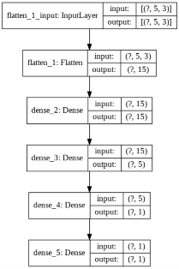
\includegraphics[width=0.3\textwidth]{./Figuras/resultados/case1_mlp2.png}
        	\caption{Topologia do modelo MLP2.} \label{fig:case1_mlp2} }
        \end{figure}
        \begin{figure}[H]
        	\center{
        		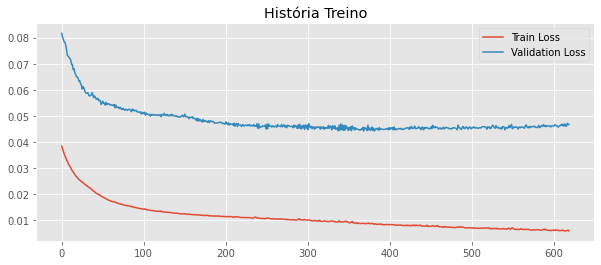
\includegraphics[width=1.0\textwidth]{./Figuras/resultados/case1_mlp2_train.png}
        	\caption{Gráfico de treino do modelo MLP2. RMSE = 107,97.}
        	\label{fig:case1_mlp2_train} }
        \end{figure}
        
    \subsection{Topologias dos melhores modelos}
    
    Nesta seção são feitos alguns comentários sobre as topologias dos modelos que obtiveram resultados, apresentados com figuras esquemáticas da rede. Para o resto dos modelos treinados, o mesmo procedimento é feito no anexo \ref{cap:anexo1}.
         
        \subsubsection{Modelo misto RNN\_EXO\_1, melhor resultado na segunda fase e em todo o trabalho}
            Interpretando o digrama do primeiro modelo misto, RNN\_EXO\_1, na Figura \ref{fig:case1_rnn_exo_1} o bloco com título GRU à esquerda na Figura de topologia do modelo, trata as entradas endógenas (temporais), assim como exemplificado nos modelos GRU endógenos. O bloco com título \textbf{Dense} é uma rede MLP que recebe um \textit{input} com 10 parâmetros de 1 dimensão, portanto todos discretos, correspondendo aos 4 parâmetros climáticos (temperatura, umidade, pressão e vento), 1 parâmetro para o dia da semana vigente, 1 para o semestre vigente e 4 parâmetros de controle do calendário (distancia da data anterior, posterior, avanço do semestre, avanço do mês). A saída dos blocos GRU e MLP são concatenadas e tratadas pelo bloco MLP de saída.
            \begin{figure}[H]
              \center{
                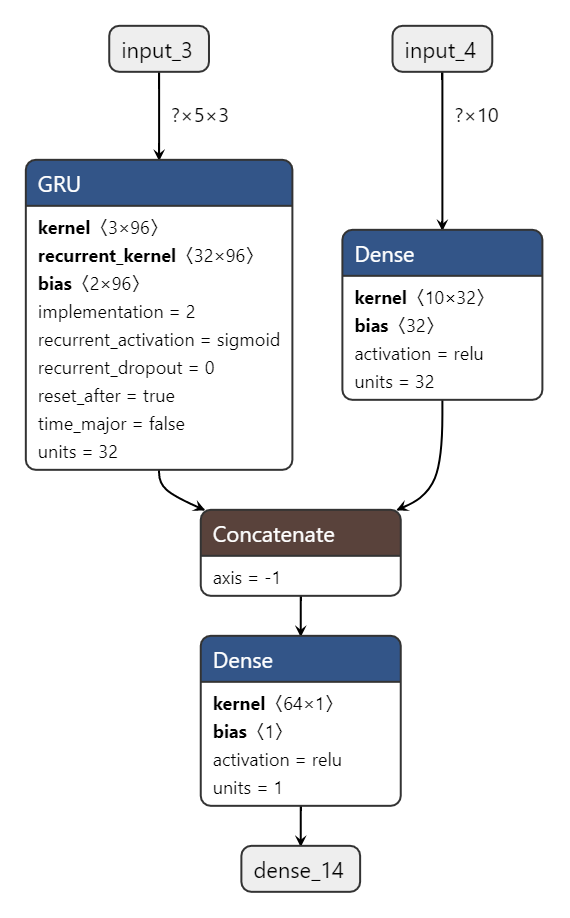
\includegraphics[width=0.7\textwidth]{./Figuras/resultados/case1_rnn_exo_1.png}
                \caption{Topologia do modelo RNN\_EXO\_1.} \label{fig:case1_rnn_exo_1} }
            \end{figure}
        %dropout
        \subsubsection{Modelo endógeno GRU RNN\_ENDO\_2, melhor resultado na primeira fase}
           Este modelo foi obtido através de uma segunda reconfiguração do primeiro modelo GRU, RNN\_ENDO\_1 detalhado na Figura \ref{fig:case1_rnn_endo1} com o aumento da profundidade de unidades deste modelo anterior, em formato regressivo de 16 unidades na primeira camada, 8 unidades na segunda e 4 na terceira, e com a inclusão do recurso \textit{dropout} fundamentado no tópico \ref{sec:drop_fund}, sua topologia final é observada na Figura \ref{fig:case1_rnn_endo2}. Este modelo produziu o melhores resultados na primeira fase experimental, detalhados na Figura \ref{fig:case1_rnn_endo2_test_dates} na próxima Seção.
            \begin{figure}[H]
              \center{
                  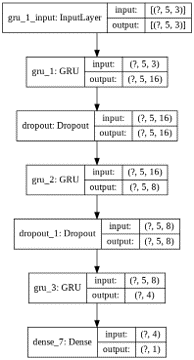
\includegraphics[width=0.24\textwidth]{./Figuras/resultados/case1_rnn_endo2.png}
                  \caption{Topologia do modelo RNN\_ENDO\_2.} 
                  \label{fig:case1_rnn_endo2} 
              }
            \end{figure}
        
    \subsection{Diferenças principais dos resultados entre as fases experimentais}
        \paragraph{Diferenças entre os melhores modelos}
        Para os experimentos da 1a fase, o modelo que produziu o menor RMSE no conjunto de testes com vantagem em todas as outras métricas foi o modelo endógeno, RNN\_ENDO\_2, com algumas anomalias de predição, como observado na Figura \ref{fig:case1_rnn_endo2_test_dates}.
        \begin{figure}[H]
          \center{
            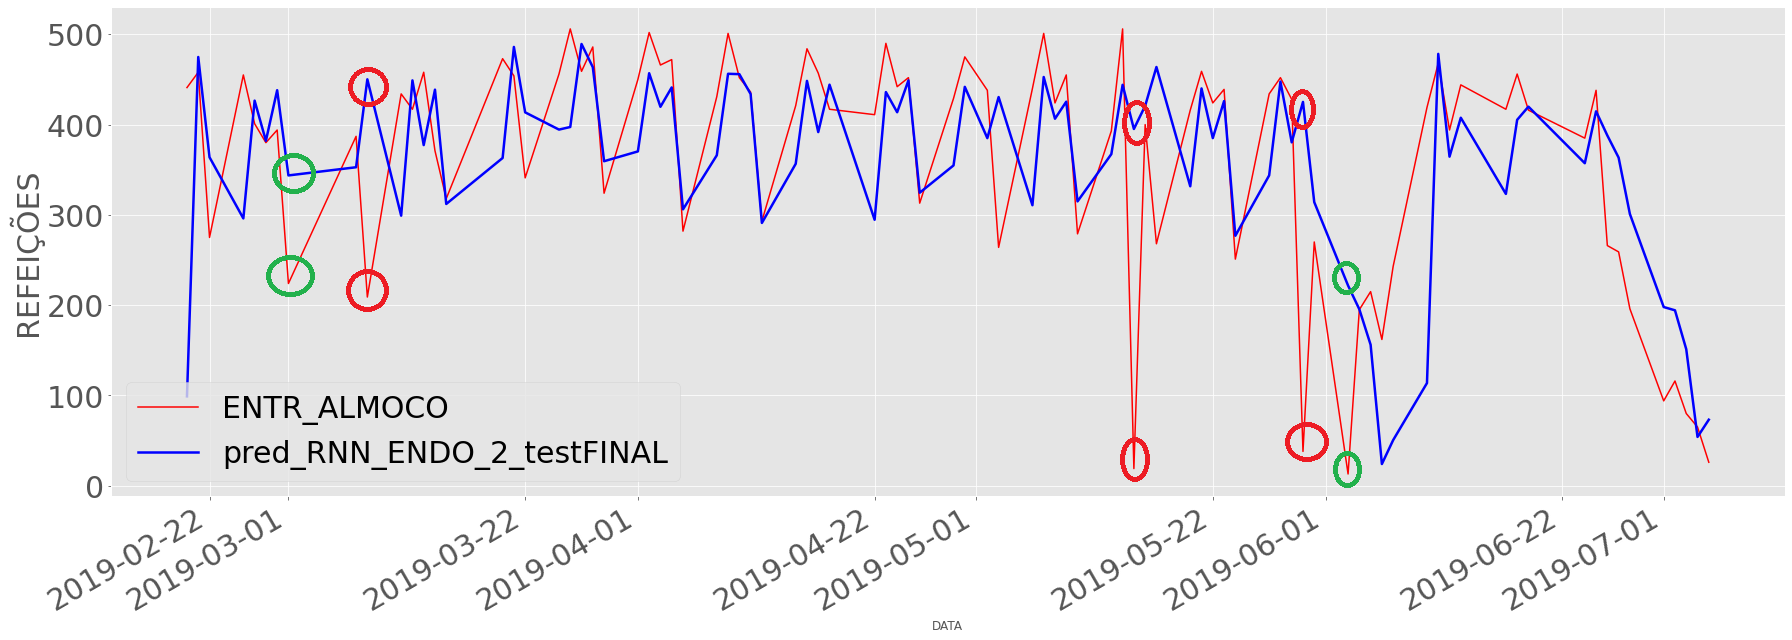
\includegraphics[width=1.0\textwidth]{./Figuras/resultados/case1_rnn_endo2_test_dates.png}
          \caption{Analise de anomalias preditivas do RNN\_ENDO\_2} \label{fig:case1_rnn_endo2_test_dates} }
        \end{figure}
        %dropout
        Os pontos verdes \textit{outliers} representam predições que corresponderam a tendência de alta ou baixa de consumo mas com erros discrepante, e os pontos vermelhos representam predições com tendência inversa ao consumo.
        As justificativas para a predição dentro da tendência, se encontram na Tabela \ref{table:rnn_endo_2_green}, denotando datas especiais que não poderiam corresponder ao processo de aprendizado do modelo.
            \begin{table}[!ht]
                \centering
                \caption{Erros de predições do modelo RNN\_ENDO\_2 na 1a fase}
                \label{table:rnn_endo_2_green}
                \rowcolors{2}{gray!25}{white}
                 \begin{tabular}{|c|c|c|}
                 \rowcolor{gray!50}
                 \hline 
                Data & Consumo & Justificativa\\ \hline    
                01/03/2019 (sexta feira)    & 224 & Sexta Feira pré - carnaval\\
                03/06/2019 (segunda feira)  &  13 & Segunda Feira pós paralisação estudantil\\ \hline 
                \end{tabular} 
            \end{table}
            
        As justificativas para previsões onde o modelo seguiu tendência oposta ao consumo também corresponderam à datas especiais, conferidas na Tabela \ref{table:rnn_endo_2_red}.
            \begin{table}[!ht]
                \caption{Anomalias de predições do modelo RNN\_ENDO\_2 na 1a fase}
                \label{table:rnn_endo_2_red}
                \rowcolors{2}{gray!25}{white}
                 \begin{tabular}{c|c|c}
                 \rowcolor{gray!50}
                 \hline
                Data & Consumo & Justificativa \\
                08/03/2019 (sexta feira)   & 209 &Sexta Feira pós - carnaval\\
                15/05/2019 (quarta feira)   & 19  & Paralisação estudantil na praça Afonso Pena\\
                30/05/2019 (quinta feira)   &  38  & Paralisação estudantil na Praça Afonso pena\\
                \hline 
                \end{tabular} 
            \end{table}
        
        Nas métricas deste modelo, é observado na Tabela \ref{table:rnn_endo_2_test} que a soma dos erros positivos, correspondeu à um descarte de aproximadamente 3479 refeições, e o erro quadrático médio de previsão foi de aproximadamente 108 refeições.
            \begin{table}[!ht]
                \centering
                \rowcolors{2}{gray!25}{white}
                \caption{Métricas do melhor modelo:  RNN\_ENDO\_2 }
                \label{table:rnn_endo_2_test}
                \begin{tabular}{c|c}
                \rowcolor{gray!50}
                \hline
                Melhor modelo: &   RNN\_ENDO\_2: \\ \hline
                Total\_Consumidas & 31962 \\ 
                Total\_Previstas & 31465,61133 \\
                Erro\_Total\_Previsao & -496,3886719 \\
                Percentual\_Erro\_Total & -1,5530\% \\\
                Correlação & 0,595439895 \\
                P-value & 9,42215E-10    \\
                RMSE &  108,0663015\\
                Soma dos erros Negativos & 2982,567947 \\
                Soma dos erros Positivos & 3478,957266\\
                ERRO\_ABS\_MEDIANO & 46,70721436 \\ 
                ERRO\_ABSOLUTO\_PERCENTUAL\_MEDIO & 74,93539002 \\ 
                \hline
                \end{tabular}
            \end{table}
        
        Já na segunda fase, todos os modelos obtiveram melhoras no erro de treino sobre o conjunto de validação, e foi obtido o modelo com as melhores predições do trabalho, o modelo misto \textbf{RNN\_EXO\_1} detalhado em sua própria Seção a seguir.
        É importante notar que as 2 fases produziram melhores modelos de classes distintas, a primeira com um modelo que utiliza apenas dados endógenos, e que contempla um conjunto de validação e teste com amplitude de apenas 1 semestre, e a segunda com um modelo que utiliza dados temporais e discretos, e que utiliza conjunto de validação e teste com amplitude de 1 ano.
        Isso denota que resultados melhores foram conquistados sem nenhuma alteração de parâmetros e hiper-parâmetros nos modelos, alterando-se apenas a organização temporal dos conjuntos de dados.
        
        Durante o teste de todos os modelos, apenas o primeiro semestre contemplou datas especiais onde estes modelos produziram anomalias de previsões, ilustrado como exemplo na Figura \ref{fig:case1_rnn_endo2_test_dates}.

\section{Resultados com o melhor modelo, RNN\_EXO\_1}
%\TODO{Nessa seção apresente os resultados do melhor modelo. Se quiser, pode dividir em subseções}
    Este modelo, representado na Figura \ref{fig:case1_rnn_exo_1} obteve os melhores resultados de todo este trabalho, quando foi treinando na segunda fase experimental.
    É notório sua melhoria de resultados com uma única mudança da organização dos conjuntos de dados entre as fases experimentais.
    
    \subsection{Comparativo do treino entre as duas fases}
   
     Nota-se que este modelo produziu convergiu à um \textit{overfitting} de forma mais lenta na primeira fase, ilustrado na Figura \ref{fig:case1_rnn_exo_1_train} em comparação ao treino da segunda fase demonstrando uma convergência à um \textit{overfitting} rápida e acentuada a partir da época 100, trazendo melhores resultados com a parada antecipada de treino, ilustrado na Figura \ref{fig:case2_rnn_exo1_train}. A diferença dos valores da métrica RMSE entre estes 2 treinos, produzindo um resultado melhor na segunda fase, de RMSE = 109,97 em comparação ao resultado da primeira fase de RMSE = 132,94.
     

        \begin{figure}[H]
        \center{                    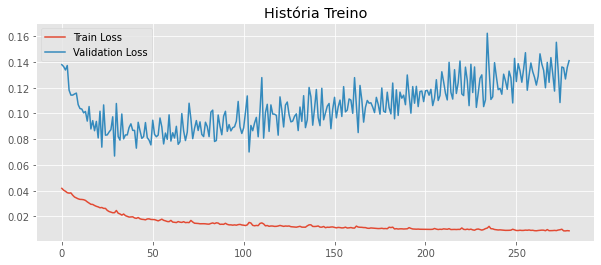
\includegraphics[width=\textwidth]{./Figuras/resultados/case1_rnn_exo_1_train.png}
        \caption{Treino do modelo RNN\_EXO\_1 na 1a fase, RMSE = 132.94} \label{fig:case1_rnn_exo_1_train} }
        \end{figure}

     

    
        \begin{figure}[H]
          \center{
            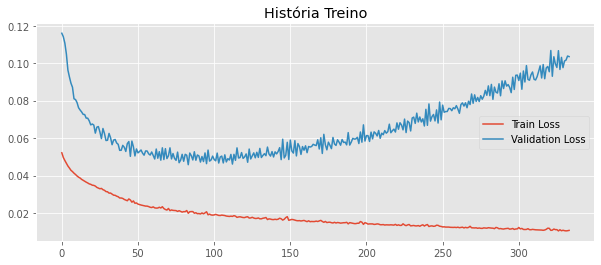
\includegraphics[width=\textwidth]{./Figuras/resultados/case2/case2_rnn_exo1_train.png}
          \caption{Gráfico de treino do modelo RNN\_EXO\_1 na 2a fase, RMSE = 109.97} \label{fig:case2_rnn_exo1_train} }
        \end{figure}
    

    \subsection{Comparativo de teste do modelo no primeiro semestre, entre as duas fases}
    
        Como este modelo treinado na segunda fase obteve os melhores resultados do trabalho, foram recalculadas as métricas para o teste de modelo dentro do domínio do primeiro semestre de 2019 para realizar uma comparação equivalente com sua versão treinada e testada também no primeiro semestre de 2019 na primeira fase.
        
        A Tabela \ref{table:case1_rnn_exo_1} demonstra que o RMSE de teste do modelo treinado na primeira fase obteve um desempenho menos satisfatório do que o RMSE treinado na segunda fase de acordo com a Tabela \ref{table:case2_rnn_exo_2_incase1}. O RMSE sendo menor no treino deste modelo na segunda fase trás uma melhoria em todas as outras métricas em comparação com o seu treino na primeira fase.
        A soma dos erros positivos de predições também foi menor na segunda fase, o que impacta menor em descarte de refeições.
        O RMSE deste modelo testado na primeira fase e alcançando RMSE = 106,208 também se saiu melhor do que o melhor modelo da primeira fase, o RNN\_ENDO\_2 que alcançou RMSE = 108,06.
        
        
        
        
        \begin{table}[!ht]
            \centering
            \caption{RNN\_EXO\_1 TREINADO NA 1A FASE,TESTE 1o SEMESTRE 2019}
            \label{table:case1_rnn_exo_1}
            \rowcolors{2}{gray!25}{white}
                \begin{tabular}{c|c}
                \rowcolor{gray!50}
                \hline
            \multicolumn{2}{c}{RNN\_EXO\_1 TREINADO NA 1A FASE,TESTE 1o SEMESTRE 2019} \\
            \hline
            RMSE & 124.49\\
            TOTAL DE REFEIÇÕES CONSUMIDAS & 31962 \\
            TOTAL DE REFEIÇÕES PROJETADAS & 28728.816  \\
            ERRO DE PREVISÃO & -3233.1839 \\
            PERCENTAGEM DE ERRO & -10.11\%  \\
            CORRELAÇÃO (r) & 0.41 \\ 
            P-value & 6.59e-05\\ 
            R2 & 0.16\\
            SOMA DOS ERROS POSITIVOS & 2709.17\\
            SOMA DOS ERROS NEGATIVOS & 5942.35\\
            ERRO ABSOLUTO MEDIANO & 85.59\\
            ERRO ABSOLUTO PERCENTUAL MÉDIO & 90.98\% \\ \hline \end{tabular} \end{table}
            
      
      
            \begin{table}[!ht]
            \centering
            \caption{RNN\_EXO\_1 TREINADO NA 2A FASE, TESTE 1o SEMESTRE 2019}
            \label{table:case2_rnn_exo_2_incase1}
            \rowcolors{2}{gray!25}{white}
                \begin{tabular}{c|c}
                \rowcolor{gray!50}
                \hline
                \multicolumn{2}{c}{RNN\_EXO\_1 TREINADO NA 2A FASE, TESTE 1o SEMESTRE 2019}\\ \hline
                RMSE & 106.2080\\
                TOTAL DE REFEIÇÕES CONSUMIDAS & 31962\\
                TOTAL DE REFEIÇÕES PROJETADAS & 32170.24\\
                ERRO DE PREVISÃO & 208.2460 \\
                PERCENTAGEM DE ERRO & 0.6515\%  \\
                CORRELAÇÃO (r)& 0.59 \\
                P-value (p) & 1.4143e-09\\
                R2 & 0.3485\\
                SOMA DOS ERROS POSITIVOS & 3454.8698\\
                SOMA DOS ERROS NEGATIVOS & 3246.6228\\
                ERRO ABSOLUTO MEDIANO & 59.5414\\
                ERRO ABSOLUTO PERCENTUAL MÉDIO & 83.2671\% \\ \hline
            \end{tabular}
            \end{table}
                
            
            
        O gráfico de dispersão do modelo treinado na primeira fase, conforme Figura \ref{fig:case1_rnn_exo_1_test_scatter} também se saiu pior, mais distante da borda superior direita do gráfico, em relação a dispersão do modelo treinado na segunda fase conforme a Figura \ref{fig:case2_rnn_exo2_test_incase1_Figura}.
        
                \begin{figure}[H]
                      \center{                    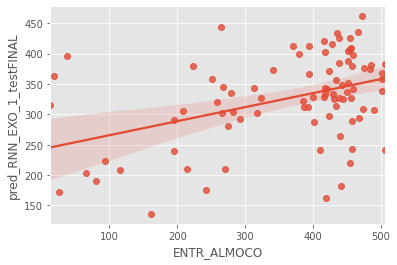
\includegraphics[width=\textwidth]{./Figuras/resultados/case1_rnn_exo_1_test_scatter.png}
                        \caption{Gráfico de dispersão de teste do modelo RNN\_EXO\_1, 1a fase} \label{fig:case1_rnn_exo_1_test_scatter} }
                        \end{figure}        
        


     \begin{figure}[H]
              \center{
                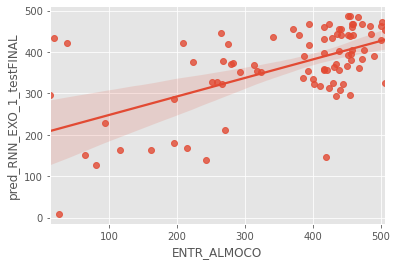
\includegraphics[width=\textwidth]{./Figuras/resultados/case2/case2_rnn_exo2_test_incase1_scatter.png}
              \caption{Gráfico de dispersão de teste do primeiro semestre, RNN\_EXO\_1 treinado na segunda fase.} \label{fig:case2_rnn_exo2_test_incase1_Figura} }
                \end{figure}        Por fim na comparativa entre os gráficos de predição, o modelo RNN\_EXO\_1 treinado na primeira fase produziu predições piores, e não aprendeu a sazonalidade semanal do consumo, como pode ser observado na Figura \ref{fig:case1_rnn_exo_1_test}, é possível notar também, na Tabela  \ref{table:case1_rnn_exo_1}, que a correlação entre os valores previstos e o consumo real, bem como o valor $R^2$ foi inferior em comparação às métricas do modelo treinado na segunda fase, e que este modelo treinado na segunda fase aprendeu melhor a sazonalidade semanal e mensal do consumo como pode ser observado na Figura \ref{fig:case2_rnn_exo2_test_incase1}.
      
           
                  \begin{figure}[H]
                      \center{                    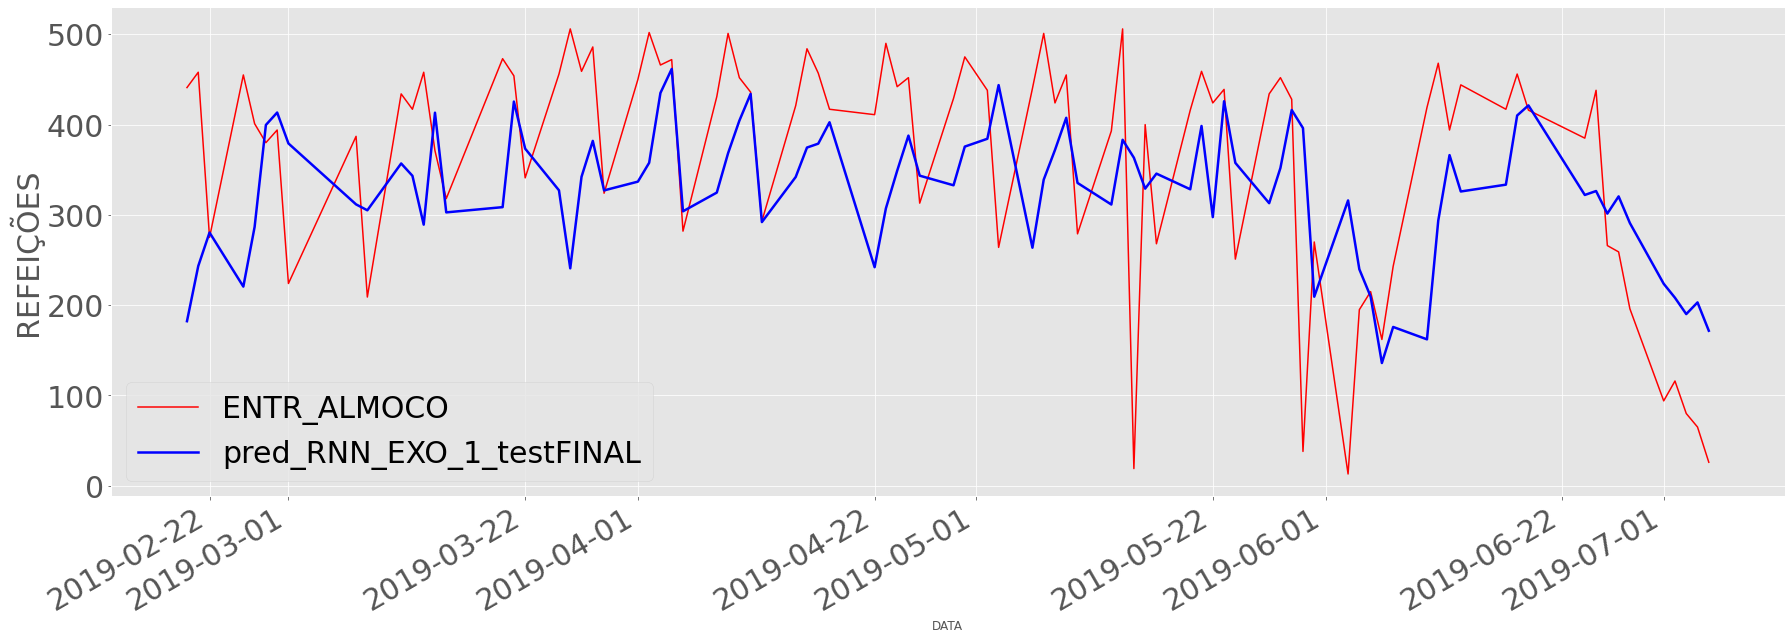
\includegraphics[width=\textwidth]{./Figuras/resultados/case1_rnn_exo_1_test.png}
                      \caption{Teste do modelo RNN\_EXO\_1, 1a fase.} 
                      \label{fig:case1_rnn_exo_1_test} }
                    \end{figure} 

   

            
            
      
           
           
            \begin{figure}[H]
              \center{
                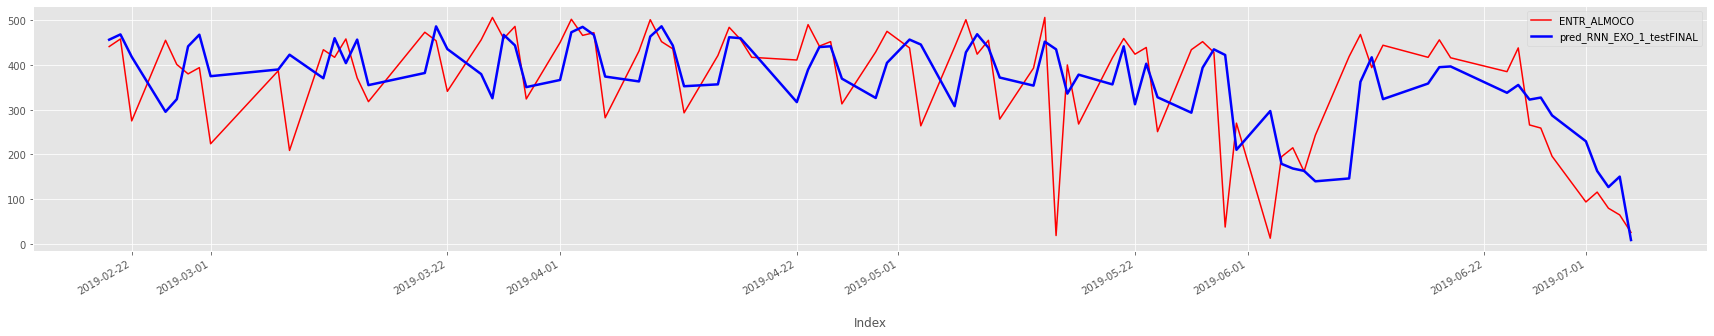
\includegraphics[width=\textwidth]{./Figuras/resultados/case2/case2_rnn_exo2_test_incase1.png}
              \caption{Teste do primeiro semestre do RNN\_EXO\_1 treinado na segunda fase.} \label{fig:case2_rnn_exo2_test_incase1} }
            \end{figure}
           
           
           
                
                
                
    \subsection{Teste final do modelo RNN\_EXO\_1 para as predições no RU do ICT-Unifesp}
    
     O teste final do modelo RNN\_EXO\_1 por fim produziu os melhores resultados com seu treino na segunda fase e sendo testado para o ano inteiro de 2019. O RMSE observado na Tabela \ref{table:case2_rnn_exo_2_2019} foi notoriamente inferior à todos os modelos treinados e testados em todo o trabalho.
     
      
        \begin{table}[!h]
            \centering
            \caption{RNN\_EXO\_1 TREINADO NA 2A FASE, TESTE ANO DE 2019}
            \label{table:case2_rnn_exo_2_2019}
            \rowcolors{2}{gray!25}{white}
                \begin{tabular}{c|c}
                \rowcolor{gray!50}
                \hline
                \multicolumn{2}{c}{RNN\_EXO\_1 TREINADO NA 2A FASE, TESTE ANO DE 2019}\\ \hline
                RMSE & 99.36\\
                TOTAL DE REFEIÇÕES CONSUMIDAS & 58653 \\
                TOTAL DE REFEIÇÕES PROJETADAS & 62048.04\\
                ERRO DE PREVISÃO & 3395.04 \\
                PERCENTAGEM DE ERRO & 5.78\%  \\
                CORRELAÇÃO (r)& 0.67 \\
                P-value (p) & 3.29e-25\\
                R2 & 0.45\\
                SOMA DOS ERROS POSITIVOS & 8163.18\\
                SOMA DOS ERROS NEGATIVOS & 4768.13\\
                ERRO ABSOLUTO MEDIANO & 55.23\\
                ERRO ABSOLUTO PERCENTUAL MÉDIO & 83.2671\% \\ \hline
            \end{tabular}
            \end{table}

    \newpage
     O descarte de refeições foi obtido pela soma dos erros positivos atingiu o valor de 4768 refeições.
     É possível notar na Figura \ref{fig:case2_rnn_exo1_test} que o modelo aprendeu bem a sazonalidade mensal e semanal do consumo, mas obteve erro discrepante para o primeiro valor previsto do segundo semestre, o erro foi justificável pois seu conjunto de treino contempla apenas 1 ano com 1 alternância de semestre impossibilitando um aprendizado melhor sobre este comportamento.
     O gráfico de dispersão ilustrado na Figura \ref{fig:case2_rnn_exo1_test_scatter} também demonstra uma boa regressão linear sobre os valores previstos pelo modelo e o valor real de consumo, se aproximando da função identidade de uma previsão ideal.
     
            %%% RNN_EXO_1
        \begin{figure}[H]
          \center{
            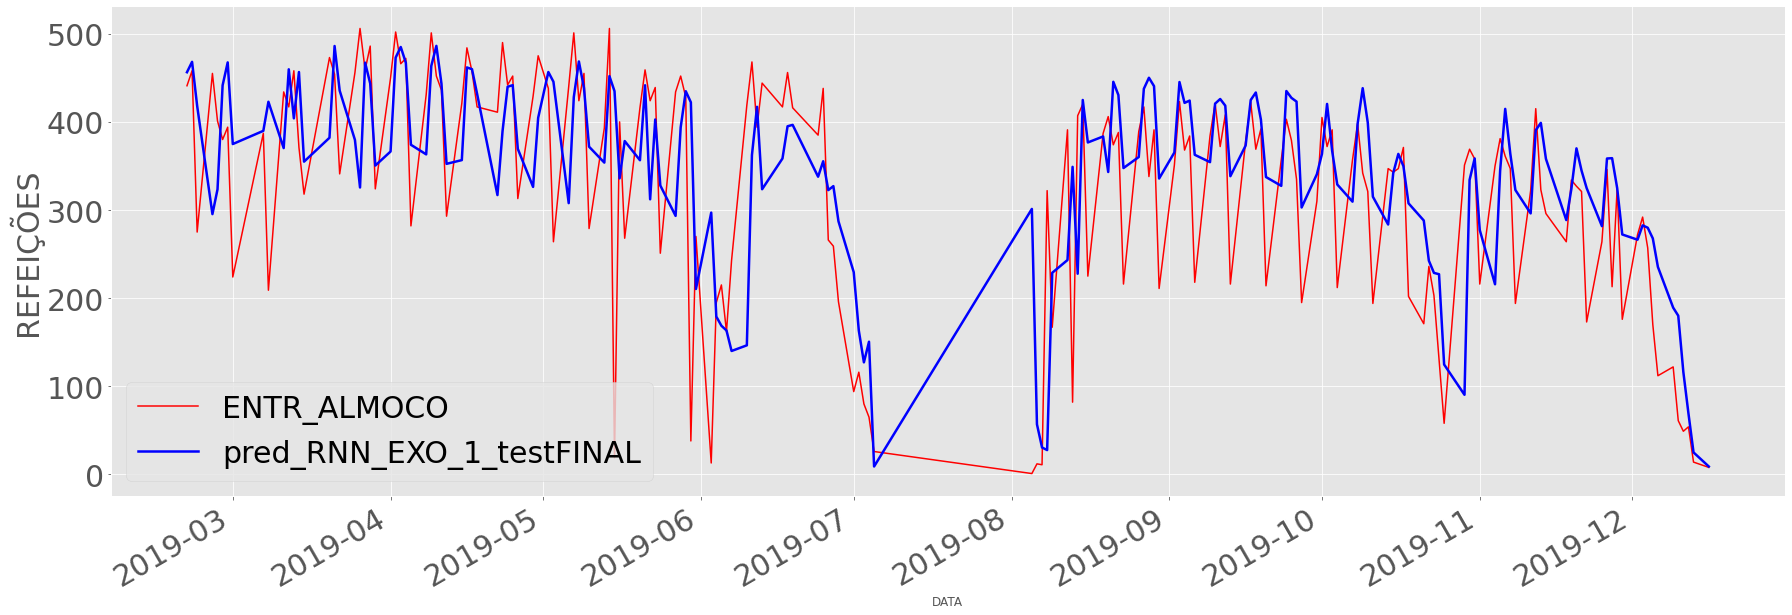
\includegraphics[width=\textwidth]{./Figuras/resultados/case2/case2_rnn_exo1_test.png}
          \caption{Gráfico final de teste do modelo RNN\_EXO\_1.} \label{fig:case2_rnn_exo1_test} }
        \end{figure}
       
       
        \begin{figure}[H]
          \center{
            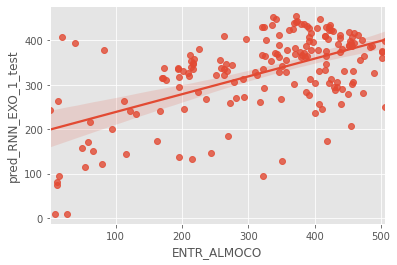
\includegraphics[width=\textwidth]{./Figuras/resultados/case2/case2_rnn_exo1_test_scatter.png}
          \caption{Gráfico de dispersão do modelo  RNN\_EXO\_1.} \label{fig:case2_rnn_exo1_test_scatter} }
        \end{figure}
        
        Resultados obtidos pelos outros métodos testados estão disponíves no \ref{chapter:outros}.
       
